\documentclass[11pt, a4paper]{article}

\usepackage{amsmath}
\usepackage{amssymb}
\usepackage{graphicx}
\usepackage{listings}
\usepackage{color}
\usepackage[section]{placeins}
\usepackage{paralist}
\usepackage{fullpage}
\usepackage{glossaries}

\usepackage{caption}
\usepackage{subcaption}

\newcommand*{\titleGM}{\begingroup
\hbox{ 
\hspace*{0.2\textwidth} 
\rule{1pt}{\textheight} 
\hspace*{0.05\textwidth} 
\parbox[b]{0.75\textwidth}{ 

{\noindent\Huge\bfseries iOS Welsh Vocabulary App}\\[2\baselineskip] % Title
{\large \textit{SEM2220 Assignment 2}}\\[4\baselineskip] % Tagline or further description
{\Large \textsc{Alexander D Brown (adb9)}} % Author name

\vspace{0.5\textheight} 
}}
\endgroup}


\begin{document}
\titleGM 
\tableofcontents
\newpage

\section{Introduction}

This report shows the process undertaken to make the pre-existing iOS Welsh Vocabulary Application to meet the following features requests:

\begin{enumerate}
\item Adding fields to the word link.
\item Updating the custom cell.
\item Adding word link detail screen.
\item Revision game.
\end{enumerate}

The existing application provides the basic functionality to display words from a SQLite database as well as the loading and saving of a single translation with no context, area or notes to the database.


\section{Development}

This section describes the process taken to implement the four feature requests required of the application, as well as detailing the problems encountered and how they were solved.

Finally this section also discusses the extra features implemented to improve the user experience.

\subsection{Implementation of Feature Requests}

This section describes how each of the four feature requests were added to the existing application.

\subsubsection{FR1: Adding Fields to the Word Link}

The first task was to allow users to add the following extra details:

\begin{itemize}
\item Context
\item Area
\item Note
\end{itemize}

All these fields were added as properties of the WordPair object.

The context is a simple, single line string, which, like the English and Welsh fields, could be added as a single text field in the UI and required altering the Word Link table to add a context column with type text.

The area can be one of three items:

\begin{itemize}
\item North
\item South
\item Both
\end{itemize}

The iOS segment selector was the perfect tool for displaying this information in the UI (with the default of Both).

An enumeration was created in code to store this information, with methods to translate from a String or character to the enumeration construct and vice versa.

In the database this information was represented as text for simplicity, it could also have been represented as a character if optimisation was an issue.

Additional methods in the \texttt{WordPair} class to translate numbers (which the segment control produces) to the enumeration type.

Finally user notes were added as a text input field and were added to the database as a text field.


\subsubsection{FR2: Update the Custom Table Cell}

The next feature was to update the table cell to display Word Link information. I went with a very simple representation, only displaying the word and all its possible translations.

\subsubsection{FR3: Add Word Link Detail Screen}

The next requirement was to show the details of a word link on a next screen.

To show this information a second table was design, showing each translation with the context of that translation.

The user can then click on these cells to show the same information that was given to add words, using a screen laid out similarly to the add words screen.

\subsubsection{FR4: Create Word Games}

Two word games were implemented, one was a simple game to select the translation from a list which contained the correct translation.

The other game is based on the popular game hangman, but gives the translated word as a clue (but trades this off with fewer guesses).

\paragraph{Translation Word Game}\hfill

The translation game requires users to pick the correct translation from four possible words. This process happens ten times and a score is shown at the end.

Rather than load the ten words before the game starts, it seemed easier to select the four word pairs from the database and then randomly select the correct word to display. This does allow duplication of questions, but allows a database size of anything greater than four to be used.

To display the four choices, a \texttt{UIPickerView} was implemented and the \texttt{TranslationGameViewController} was also made a delegate for this picker. To make this process easier, the correct position of the word in the array the picker uses is stored and then used to check if the choice is correct.

Initially, the idea of seguing back to the same view was considered, but it was found that simply manipulating the view dynamically was much easier to deal with.

To segue at the end of the game two different buttons are used. The first is visible through the entire game until the last question, at which point it becomes hidden and another, previously hidden, button is made visible to perform the segue to the results page.

\paragraph{Hangman Game}\hfill

The hangman game was marginally easier to implement, but did bring about some more radical changes to existing code.

Previously, the translation game had handled the random selection of words but, with another class which needed to perform the exact same logic, this code was moved into the \texttt{SharedData} class. This keeps the concerns of loading data in a single place.

It also affected the \texttt{WordPair} class to have better methods for providing words in different languages. Previously a few helper methods had been implemented to get a word from a certain language and the translation from a certain language, required because both games would only know the language the answer was in.

This mean that guessing the Welsh word also involved guessing the context (including brackets and spaces). This was changed to pass in a boolean requesting the context.

The images were displayed in a \texttt{UIImageView} and were loaded into an array when the view loads. A call to the methods to set the image for the view was then used with the index of the image to display which corresponded to the number of lives the user had left.

\subsection{Problems Encountered}

Some of the main problems encountered in this project were due to the lack of familiarisation with Objective C and the iOS framework. Sites like the iOS documentation and StackOverflow were used to gain knowledge of what should be done to solve a problem and how to debug common problems.

One problem that was found was more of a C issue than an Objective C problem; circular dependencies.

The initial code has the language setting enumeration in the \texttt{SharedData} class, which includes the \texttt{WordLink} header which, in turn, includes the \texttt{WordPair} header.

Later in the project the language settings were needed in the \texttt{WordLink} class to provide extra functionality required for the feature requests. At this point the \texttt{WordLink} header also included the \texttt{SharedData} header. This made the enumeration inaccessible in the \texttt{WordLink} header despite the fact it would seem it should be.

Initially a C style fix was employed using macros, but this was quickly remedied by moving the enumeration into the \texttt{WordLink} header, and later into the \texttt{WordPair} header for similar reasons.


\section{Testing}

This section describes the testing performed on the application, specifically using the iOS simulator.

Figure~\ref{fig:add-words} shows the screen the user would use to add new words to the database and also how their input is checked to make sure the English or Welsh field is not blank.

\begin{figure}[h]
\centering
\begin{subfigure}[b]{0.3\textwidth}
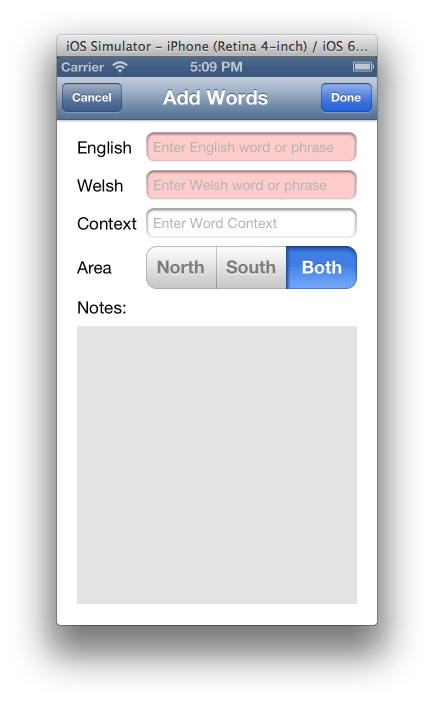
\includegraphics[width=\textwidth]{img/add-word-init}
\caption{Initial Add Words Screen}
\end{subfigure}
\begin{subfigure}[b]{0.3\textwidth}
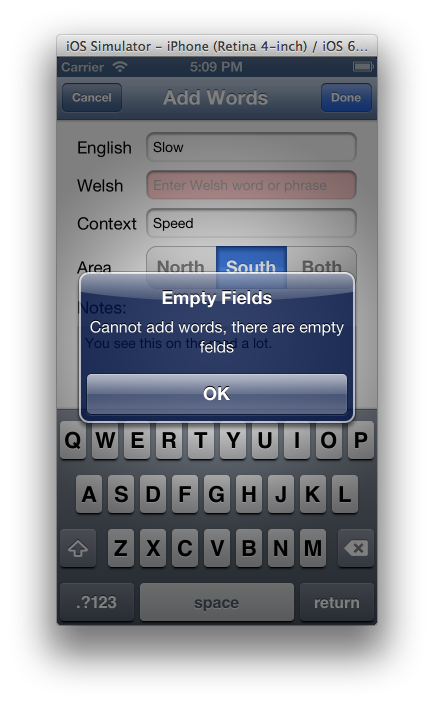
\includegraphics[width=\textwidth]{img/add-word-error}
\caption{Error Checking}
\end{subfigure}
\caption{Allowing the User to Add Words}
\label{fig:add-words}
\end{figure}

Figure~\ref{fig:display-words} shows the screens which display existing words to the user. As most of this functionality is produced directly from database queries and using the storyboard elements, there is very little testing that can actually be performed on it, other than checking the correct words are loaded.

\begin{figure}[h]
\centering
\begin{subfigure}[b]{0.3\textwidth}
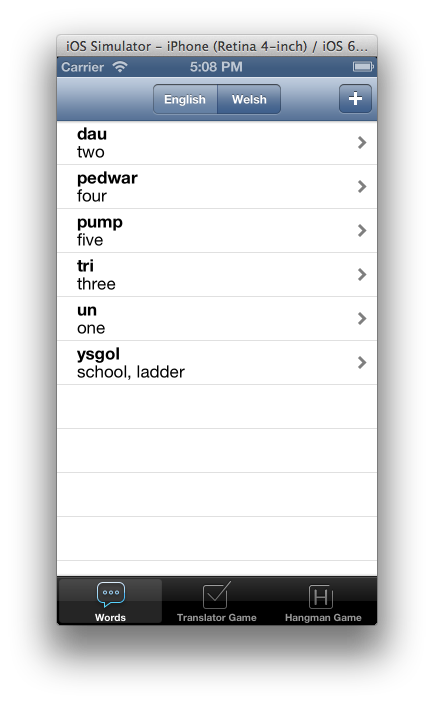
\includegraphics[width=\textwidth]{img/words-list}
\caption{The Words List Screen}
\end{subfigure}
\begin{subfigure}[b]{0.3\textwidth}
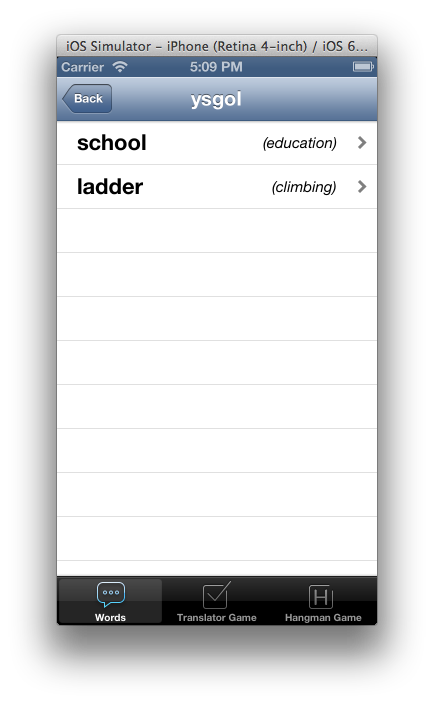
\includegraphics[width=\textwidth]{img/word-link}
\caption{The Word Link Screen}
\end{subfigure}
\begin{subfigure}[b]{0.3\textwidth}
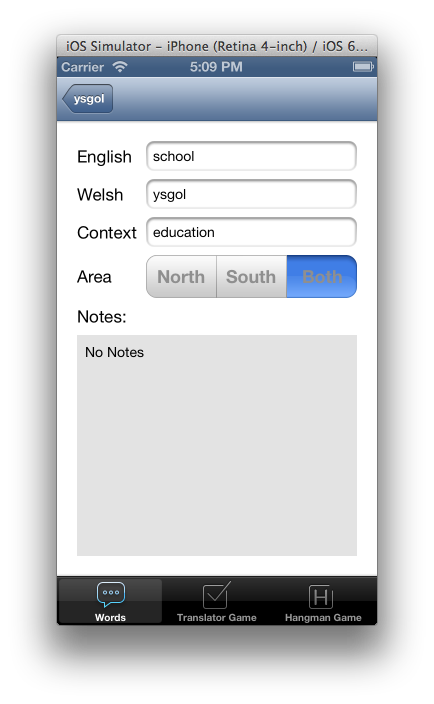
\includegraphics[width=\textwidth]{img/word-detail}
\caption{The Word Detail Screen}
\end{subfigure}
\caption{Displaying Words to the User}
\label{fig:display-words}
\end{figure}

Figure~\ref{fig:trans-game} shows the Translation game in progress. Again this is mostly handled by database interaction and storyboard elements. To test a number of questions were answered correctly to ensure the scoring worked as expected.

\begin{figure}[h]
\centering
\begin{subfigure}[b]{0.3\textwidth}
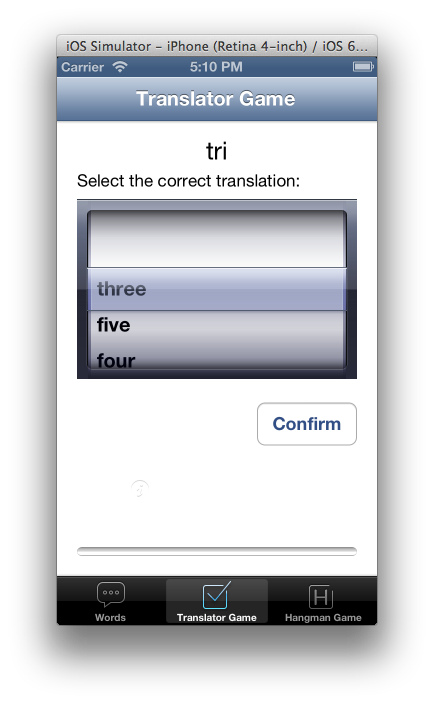
\includegraphics[width=\textwidth]{img/trans-game}
\caption{Presenting the Question}
\end{subfigure}
\begin{subfigure}[b]{0.3\textwidth}
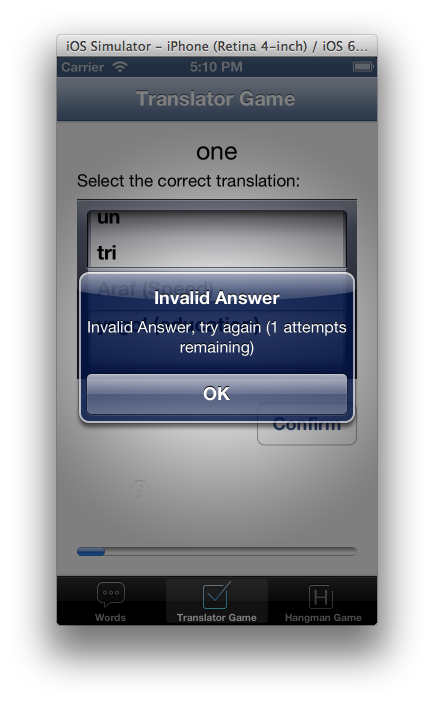
\includegraphics[width=\textwidth]{img/trans-game-error}
\caption{Getting an Answer Wrong}
\end{subfigure}
\begin{subfigure}[b]{0.3\textwidth}
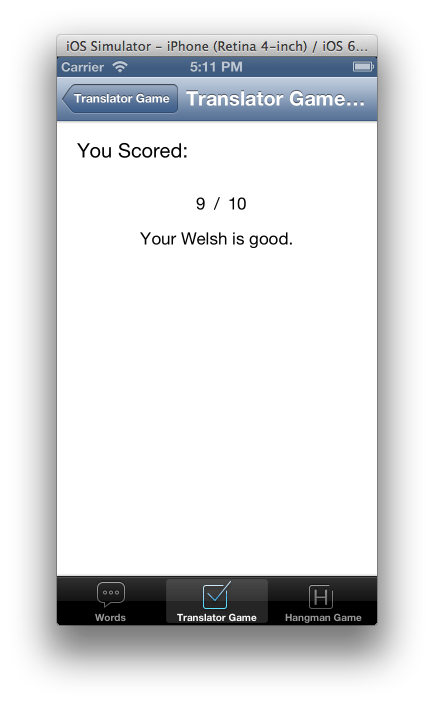
\includegraphics[width=\textwidth]{img/trans-game-results}
\caption{Results}
\end{subfigure}
\caption{The Translation Game at Different Points in the Game}
\label{fig:trans-game}
\end{figure}

Figure~\ref{fig:hangman-game} shows the Hangman game in progress. As with the Translation game the only real way to test this was to play the game several times making a mixture of correct and incorrect decisions.

\begin{figure}[h]
\centering
\begin{subfigure}[b]{0.3\textwidth}

\includegraphics[width=\textwidth]{img/hangman}
\caption{Presenting the Question}
\end{subfigure}
\begin{subfigure}[b]{0.3\textwidth}
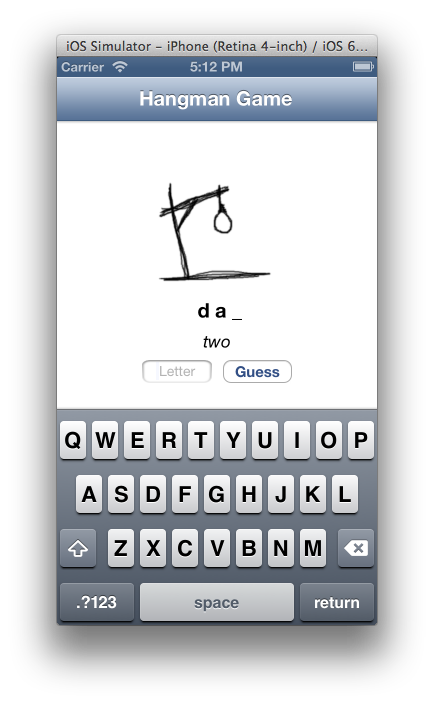
\includegraphics[width=\textwidth]{img/hangman-prog}
\caption{In Progress}
\end{subfigure}
\\
\begin{subfigure}[b]{0.3\textwidth}
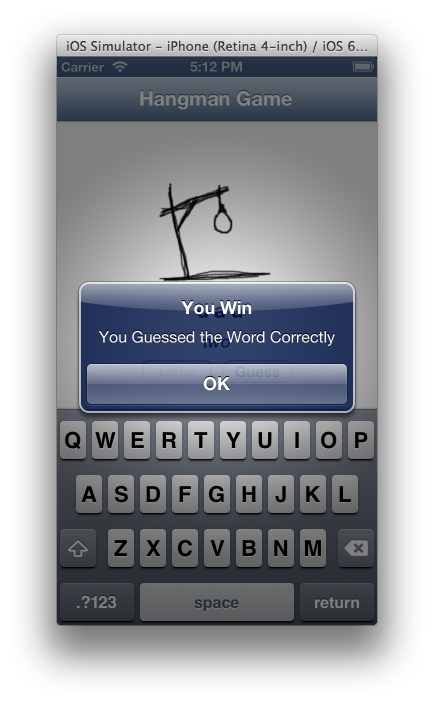
\includegraphics[width=\textwidth]{img/hangman-win}
\caption{Winning the Game}
\end{subfigure}
\begin{subfigure}[b]{0.3\textwidth}
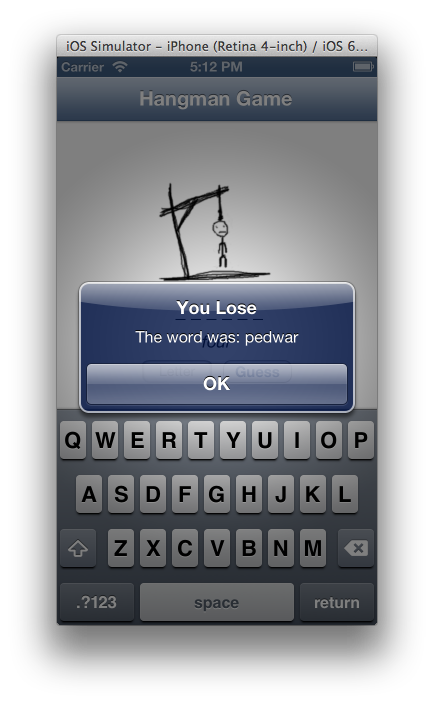
\includegraphics[width=\textwidth]{img/hangman-lose}
\caption{Losing the Game}
\end{subfigure}
\caption{The Hangman Game at Different Points in the Game}
\label{fig:hangman-game}
\end{figure}

\section{Evaluation}

All of the feature request have been implemented and evidenced as per the figures show in the previous section. The code is of somewhat decent quality; due to a lack of familiarity of Objective-C it is, perhaps, not as slick as it could be. As well as this, a lot of the code has been put into the View Controller classes when it could have been isolated into separate classes.

Where possible code was refactored out of the view controllers and into the data access classes when the functionality was either repeated or long winded.

The author has learnt a lot about the process taken to develop iOS applications, as well as the API for many of the objects used in both iOS applications and the standard Objective-C libraries. Aside from this, the author has tried to take the time to learn some of the standards for developing iOS applications, one notable part of this was to use the \texttt{arc4random} random number generator rather than the standard \texttt{random} random number generator as it actually begins to provide true randomness without the need for providing a decent method of seeding the generator.

Much of the development took the same process any other project would have, slowly developing and testing each feature, using the documentation where needed. The documentation provided by Apple in XCode was generally enough to find out the use of any User Interface object which were needed and where this was not enough, online help sites generally had a related query which could be adapted to suit the needs of the project.

The author does feel that iOS development relies too heavily on XCode, especially when basic tasks like editing the XML descriptor of the user interface is actively discouraged. Objective-C does seem like a powerful language with lots of useful libraries, but the author found the verboseness of it tended to make finding the correct method calls more difficult, especially given some of the fairly standard naming used by other languages. 

Breaking down the mark scheme the author has predicted the grade which should be given for each part, this is shown in table~\ref{tab:marks}.

Therefore, the author feels a mark of 82\% should be awarded. The values chosen were based on the following reasons:

\begin{description}
\item[Documentation] This report gives details of the process taken to build the iOS Welsh Vocabulary Application, the problems encountered during this process, what was learned during this project and this indication of which mark should be awarded.
\item[Implementation] All the feature request were implemented and the design, code and database structure now meet functionality needed to implement these feature request. The implemented code uses sensible names and structure and errors are caught and handled where needed.
\item[Flair] The hangman and translation games both use element which allow them to be displayed in a very user friendly way.
\item[Testing] No testing was done using browser developer tools and the author wonders why the specification asks for these tools to be used for a native phone application. Despite this, testing has been performed using the iOS simulator and evidence has been produced in the testing section.
\end{description}

\begin{table}[h]
\centering
\begin{tabular}{|c|c|c|}\hline
\textbf{Part} & \textbf{Worth} & \textbf{Predicted Grade} \\ \hline
Documentation & 30\% & 25\% \\ 
Implementation & 50\% & 45\% \\ 
Flair & 10\% & 5\% \\ 
Testing & 10\% & 7\% \\ \hline
Total & 100\% & 82\% \\ \hline
\end{tabular}
\caption{Break Down of Marks}\label{tab:marks}
\end{table}

\newpage

\end{document}
